Within the theory of continuum mixture theory, a poroelastic medium is treated as the superposition of
two interacting continua simultaneously occupying the same physical space. The
superscript $\alpha \in {s, f}$ denotes a quantity related to the solid or fluid.  Before presenting the mixture theory, we give a review of solid mechanics. This will form the basis of the description of the solid skeleton. The following review of continuum mechanics closely follows chapter 4 in \citet{gonzalez2008first}, and the standard Poromechanics book by \citet{coussy2004poromechanics}. Most of the kinematic quantities described here will be associated with the solid skeleton, since this also describes the motion of the fluid domain.
\begin{figure}[H]
\begin{center}

 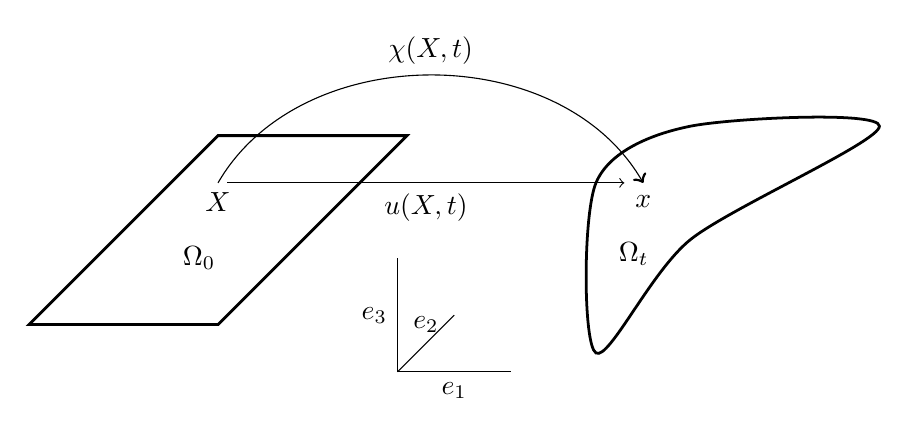
\begin{tikzpicture}[yscale=1.2,xscale=1.2,shift={(-10,0)}]
  
\draw[->] (-1,0.5) to [out=60,in=120,line width=1pt ] node[above,midway ]{$\boldsymbol{\chi}(\boldsymbol{X},t) $} ++(4.5,0) ; 

\draw[->] (-0.9,0.5) to  node[below,midway,line width=1pt  ]{$\boldsymbol{u}(\boldsymbol{X},t) $} ++(4.2,0) ; 

\draw (-1,0.3) node {{$\boldsymbol{X}$}};
\draw (3.5,0.3) node {{$\boldsymbol{x}$}};
\draw (-1.2,-0.3) node {{$\Omega_{0}$}};
\draw (3.4,-0.25) node {{$\Omega_{t}$}};

%\draw [->,line width=5pt] (-2.4,0.3) arc ;
%\draw [->,line width=5pt,smooth]  (-1,-1) -- (1,1) ;

\begin{scope}[shift={(-2,0)}]
 \draw  [line width=1pt]  (-1,-1) -- (1,1) -- (3,1)  -- (1,-1) -- cycle;
\end{scope}

\begin{scope}[shift={(1,-0.7)},yscale=.6,xscale=1]
\draw [line width=1pt]  plot [smooth cycle] coordinates {(2,2) (3,3) (5,3) (3,1) (2,-1)};
\end{scope}

%Draw the axes
%\begin{scope}[shift={(-4,-1.5)},yscale=0.6,xscale=0.6]
%\draw[-] (0,0) to node[below,midway,line width=1pt  ]{$\boldsymbol{e}_{1}  $} (2,0) ; 
%\draw[-] (0,0) to node[left,midway,line width=1pt  ]%{$\boldsymbol{e}_{3}  $} (0,2) ; 
%\draw[-] (0,0) to node[above,midway,line width=1pt  ]%{$\boldsymbol{e}_{2}  $} (1,1) ; 
%\end{scope}


\begin{scope}[shift={(0.9,-1.5)},yscale=0.6,xscale=0.6]
\draw[-] (0,0) to node[below,midway,line width=1pt  ]{$\boldsymbol{e}_{1}  $} (2,0) ; 
\draw[-] (0,0) to node[left,midway,line width=1pt  ]{$\boldsymbol{e}_{3}  $} (0,2) ; 
\draw[-] (0,0) to node[above,midway,line width=1pt  ]{$\boldsymbol{e}_{2}  $} (1,1) ; 
\end{scope}




\end{tikzpicture}
\caption{Illustration of the solid deformation.}
\label{fig:kinematic_deformation}
\end{center}
\label{fig:kinematic}
\end{figure}

\begin{comment}

 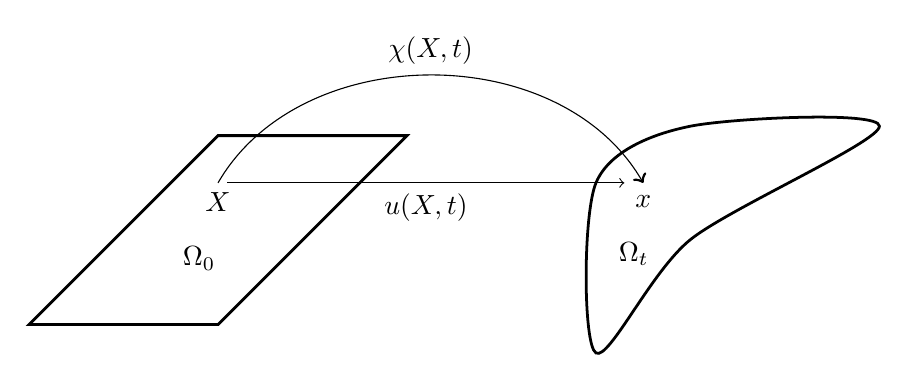
\begin{tikzpicture}[yscale=1.2,xscale=1.2,shift={(-10,0)}]
  
\draw[->] (-1,0.5) to [out=60,in=120,line width=1pt ] node[above,midway ]{$\boldsymbol{\chi}(\boldsymbol{X},t) $} ++(4.5,0) ; 

\draw[->] (-0.9,0.5) to  node[below,midway,line width=1pt  ]{$\boldsymbol{u}(\boldsymbol{X},t) $} ++(4.2,0) ; 

\draw (-1,0.3) node {{$\boldsymbol{X}$}};
\draw (3.5,0.3) node {{$\boldsymbol{x}$}};
\draw (-1.2,-0.3) node {{$\Omega_{0}$}};
\draw (3.4,-0.25) node {{$\Omega_{t}$}};

%\draw [->,line width=5pt] (-2.4,0.3) arc ;
%\draw [->,line width=5pt,smooth]  (-1,-1) -- (1,1) ;

\begin{scope}[shift={(-2,0)}]
 \draw  [line width=1pt]  (-1,-1) -- (1,1) -- (3,1)  -- (1,-1) -- cycle;
\end{scope}

\begin{scope}[shift={(1,-0.7)},yscale=.6,xscale=1]
\draw [line width=1pt]  plot [smooth cycle] coordinates {(2,2) (3,3) (5,3) (3,1) (2,-1)};
\end{scope}

\end{tikzpicture}
\caption{Illustration of the solid deformation.}
\label{fig:kinematic_deformation}
\end{center}
\label{fig:kinematic}
\end{figure}
\end{comment}

Let the volume $\Omega_{0}$ be the undeformed Lagrangian (material) reference configuration and let $\boldsymbol{X}=\lbrace X\boldsymbol{e}_{1} +Y\boldsymbol{e}_{2} + Z\boldsymbol{e}_{3} \rbrace $ indicate the position of a solid particle in $\Omega_{0}$ at $t=0$, where $X,Y$ and $Z$ are the components of the position with respect to the standard orthonormal basis $\lbrace \boldsymbol{e}_{1}  ,\boldsymbol{e}_{2}  , \boldsymbol{e}_{3}  \rbrace $ for $\mathbb{R}^{3}$. The position of a solid particle in the current Eulerian (spatial) configuration $\Omega_{t}$ is given by $\boldsymbol{x}=\lbrace x\boldsymbol{e}_{1} +y\boldsymbol{e}_{2} + z\boldsymbol{e}_{3} \rbrace$, with  $\boldsymbol{x}=\boldsymbol\chi(\boldsymbol{X},t)$, shown in Figure \ref{fig:kinematic_deformation}. The deformation map, $\boldsymbol\chi(\boldsymbol{X},t)$, is a continuously
differentiable, invertible mapping from $\Omega_{0}$ to $\Omega_{t}$. Thus the inverse of the deformation map, $\boldsymbol\chi^{-1}(\boldsymbol{x},t)$, is such that $\boldsymbol{X}=\boldsymbol\chi^{-1}(\boldsymbol{x},t)$. The displacement field is given by
\begin{equation}
 \boldsymbol{u}(\boldsymbol{X},t)=\boldsymbol\chi(\boldsymbol{X},t)-\boldsymbol{X}.
 \label{eqn:displacement}
\end{equation}
The deformation gradient tensor,
\begin{equation}
 \boldsymbol{F}=\frac{\partial \boldsymbol\chi(\boldsymbol{X},t)}{\partial \boldsymbol{X}}=\boldsymbol{I}+\frac{\partial \boldsymbol{u}(\boldsymbol{X},t)}{\partial \boldsymbol{X}} ,
 \label{eqn:deformation_gradient}
\end{equation}
maps a material line element in the reference configuration ${d}\boldsymbol{X}$, to a line element ${d}\boldsymbol{x}$ in the current configuration, i.e. ${d}\boldsymbol{x}=\boldsymbol{F}{d}\boldsymbol{X}$. The symmetric right Cauchy-Green deformation tensor is given by
\begin{equation}
\boldsymbol{C}={\boldsymbol{F}}^{T}{\boldsymbol{F}}.
\label{eqn:right_cg_tensor}
\end{equation}
The jacobian is defined as
\begin{equation}
 J=\mbox{det}(\boldsymbol{F}),
 \label{eqn:jacobian}
\end{equation}
and represents the change in an infinitesimal small volume from the reference to the current configuration. Also note that $J > 0$, to avoid self penetration of the body. We also have that $J$ represents the change in an infinitesimal small volume from a reference volume element $d \Omega_{0}$ to a currret configuration  volume element $d \Omega_{t}$
\begin{equation}
d\Omega_{t}=Jd\Omega_{0}.
\label{j_volume}
\end{equation}
Also, $\boldsymbol{F}$ is invertible, and it is easy to see that the inverse of the deformation gradient is the deformation gradient of the inverse map
\begin{equation}
\boldsymbol{F}^{-1}=\frac{\partial \boldsymbol{\chi}^{-1}(\boldsymbol{x},t)}{\partial \boldsymbol{x} }=\frac{\partial \boldsymbol{X}}{\partial \boldsymbol{x} }.
\end{equation}
\begin{comment}
$\boldsymbol{F}$ can also be used to map between surfaces in the two configurations. Consider a surface element $dA$, oriented by the unit normal vector $\boldsymbol{N}$ in the undeformed configuration, and ${d}a$, a surface element in the deformed configuration, oriented by the unit normal vector $\boldsymbol{n}$, then
\begin{equation}
 \boldsymbol{n}  {d}a=J \boldsymbol{F}^{-T}  \boldsymbol{N} dA.
\label{eqn:push_backward}.
\end{equation}
For a detailed derivation see section 4.6.3 in \cite{gonzalez2008first} (Might not actually need this for this document).
\end{comment}
%\subsection{Time derivatives}
We denote by $\boldsymbol{V}(\boldsymbol{X},t)$ the velocity at time $t$ of the material (fixed) solid particle $\boldsymbol{X}$. By definition we have
\begin{equation}
 \boldsymbol{V}(\boldsymbol{X},t)= \pderiv{}{t}\boldsymbol\chi(\boldsymbol{X},t).
\end{equation}
Similarly, we denote by $\boldsymbol{A}(\boldsymbol{X},t)$ the acceleration, given by
\begin{equation}
 \boldsymbol{A}(\boldsymbol{X},t)= \frac{\partial^{2}}{\partial t^{2}}\boldsymbol\chi(\boldsymbol{X},t).
\end{equation}
We see that the velocity and acceleration of material particles are material fields. Also note that $\pderiv{}{t}\boldsymbol{u}(\boldsymbol{X},t)=\pderiv{}{t}\boldsymbol\chi(\boldsymbol{X},t)$. We will also require a spatial description of these fields. We denote by $\boldsymbol{v}^{s}(\boldsymbol{x},t)$ the spatial description of the material solid velocity field, such that
\begin{equation}
\label{eqn:vs_spatial}
 \boldsymbol{v}^{s}(\boldsymbol{x},t)= \left. \left[ \pderiv{}{t}\boldsymbol\chi(\boldsymbol{X},t) \right] \right|_{\boldsymbol{X}={\chi}^{-1}(\boldsymbol{x},t)}.
\end{equation}
Similarly, for the spatial description of the solid acceleration, we have
\begin{equation}
 \boldsymbol{a}^{s}(\boldsymbol{x},t)= \left. \left[ \frac{\partial^{2}}{\partial t^{2}}\boldsymbol\chi(\boldsymbol{X},t) \right] \right|_{\boldsymbol{X}={\chi}^{-1}(\boldsymbol{x},t)}.
\end{equation}
Notice that $\boldsymbol{v}^{s}(\boldsymbol{x},t)$ and $\boldsymbol{a}^{s}(\boldsymbol{x},t)$ correspond to the velocity and acceleration of the solid material particle whose current coordinates are $\boldsymbol{x}$ at time $t$. Also note that by definition of $\boldsymbol{v}^{s}$ in (\ref{eqn:vs_spatial}) we have (see \citep[page 132]{gonzalez2008first})
\begin{equation}
 \left. \boldsymbol{v}^{s}(\boldsymbol{x},t)
\right|_{\boldsymbol{x}=\boldsymbol{\chi}(\boldsymbol{X},t)} =  \pderiv{}{t}\boldsymbol{\chi}(\boldsymbol{X},t) .
\label{eqn:spatial_velocity}
\end{equation}
%\subsubsection{The Reynolds transport theorem for mixtures velocity and acceleration}
%For a spatial field $\boldsymbol{w}^{s}=\boldsymbol{w}^{s}(\boldsymbol{x},t)$ associated with the solid skeleton, the particle derivative is defined as 
%\begin{equation}
%\frac{d^{s} \boldsymbol{w}^{s}}{dt}=\pderiv{}{t}\boldsymbol{w}^{s} + %(\nabla\boldsymbol{w}^{s})\boldsymbol{v}^{s},
%\label{eqn:particle_deriv_s}
%\end{equation}
%where $\nabla( \cdot)= \frac{\partial (\cdot) }{\partial \boldsymbol{x} } $ denotes the %partial derivative with respect to $\boldsymbol{x}$. Since nearly all our workings will be %performed in the current configuration we will keep the shorthand notation $\nabla$ to %denote the spatial gradient in the current configuration instead of explicitly writing  %$\nabla_{\boldsymbol{x}}$. For a spatial field %$\boldsymbol{w}^{f}=\boldsymbol{w}^{f}%(\boldsymbol{x},t)$, associated with the fluid, the particle derivative following the %motion of the fluid is defined by (see eqn. (3.9) in \cite{boer2005trends})
%\begin{equation}
%\frac{d^{f} \boldsymbol{w}^{f}}{dt}=\pderiv{}{t}\boldsymbol{w}^{f} + %(\nabla\boldsymbol{w}^{f})\boldsymbol{v}^{f}. 
%\end{equation}
%Here $\boldsymbol{v}^{f}$ is the velocity of the fluid. 
The \textbf{particle derivative of a field} $\mathcal{G}(\boldsymbol{x},t)$ with respect to the particle $\alpha$ ($s$ or $f$) is given by (see \citep[eqn. (1.43)]{coussy2004poromechanics})
\begin{equation}
\frac{d^{\alpha}}{dt} \mathcal{G}=\pderiv{\mathcal{G}}{t}  + (\nabla\mathcal{G})\boldsymbol{v}^{\alpha},
\end{equation}
where $\nabla( \cdot)= \frac{\partial (\cdot) }{\partial \boldsymbol{x} } $ denotes the partial derivative with respect to $\boldsymbol{x}$. Since nearly all our workings will be performed in the current configuration we will keep the shorthand notation $\nabla$ to denote the spatial gradient in the current configuration instead of explicitly writing  $\nabla_{\boldsymbol{x}}$. The \textbf{particle derivative of a material volume} with respect to the $\alpha$-constituent is given by (see \citep[eqn. (1.42)]{coussy2004poromechanics})
\begin{equation}
\frac{d^{\alpha}}{dt} (d \Omega_{t})=\left(\nabla \cdot \boldsymbol{v}^{f}   \right)d \Omega_{t}. 
\end{equation}
The particle derivative also applies to a volume integral. Thus, for any quantity $\mathcal{G}$, associated with the $\alpha$ constituent, we have (see \citep[eqn. (1.47)]{coussy2004poromechanics})
\begin{equation}
\label{eqn:reynolds_transport}
\frac{d^{\alpha}}{dt} \int_{\Omega_{t}} \mathcal{G} d \Omega_{t} =  \int_{\Omega_{t}} \frac{d^{\alpha}}{dt}(\mathcal{G} d \Omega_{t})= \int_{\Omega_{t}} \left( \frac{d^{\alpha}\mathcal{G}}{dt} + \mathcal{G} \nabla \cdot \boldsymbol{v}^{\alpha} \right) d \Omega_{t}= \int_{\Omega_{t}} \left( \frac{\partial \mathcal{G}}{ \partial t} +  \nabla \cdot \mathcal{G} \boldsymbol{v}^{\alpha} \right) d \Omega_{t}.
\end{equation}
This is commonly known as the Reynolds transport theorem, in the last step we have used the identity  $\nabla \cdot (\psi \boldsymbol{s}) =  \boldsymbol{s} \cdot \nabla \psi + \psi \nabla \cdot \boldsymbol{s} $ for some scalar $\psi$ and vector $\boldsymbol{s}$.